% methodsandresults.tex

\begin{figure}
\setlength{\abovecaptionskip}{0pt}
\setlength{\belowcaptionskip}{0pt}
\centering
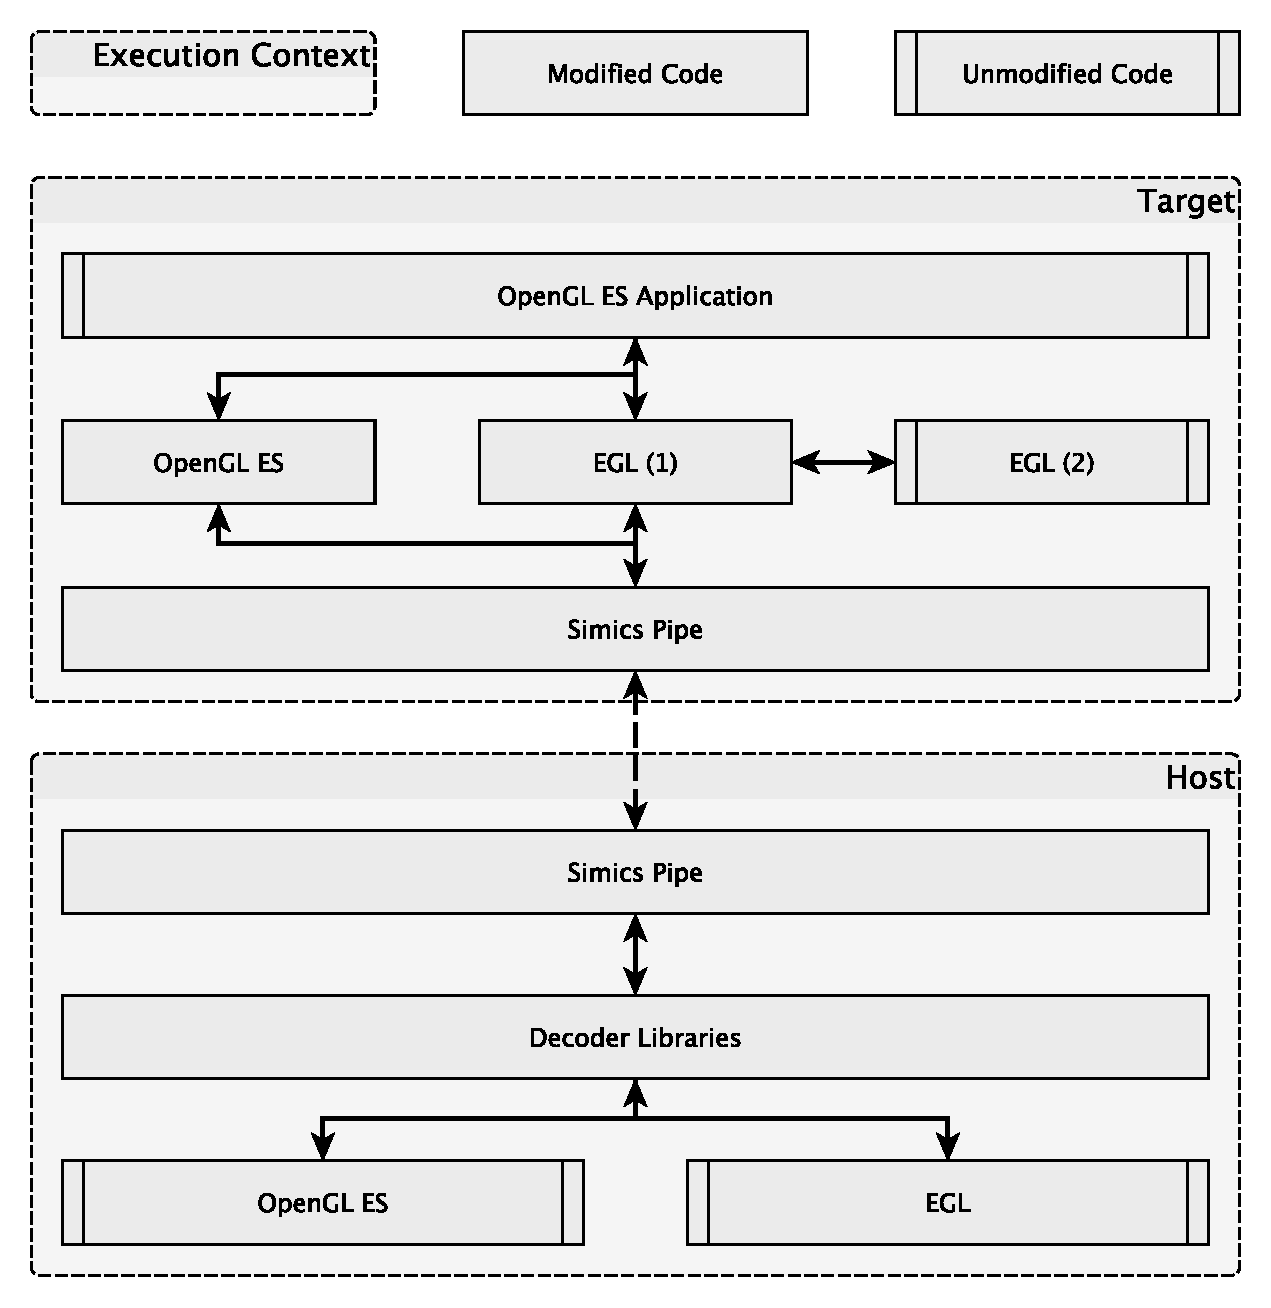
\includegraphics[width=\linewidth]{img/yedoverview.pdf}
\caption{Overview of paravirtualized graphics in Simics.}
\label{fig:overview}
\end{figure}

% Methods and Results
\section{Methods and Results}
\label{sec:methodsandresults}
OpenGL paravirtualization in Simics encompasses three overall components, being the target system libraries, the host system libraries, and a communications channel between them named the "Simics pipe".
To facilitate easier development, target and host system libraries may be partly generated from specification files detailing function signatures and arguments.
Except methods that require state saving, the majority of the libraries are generated this way.

The generated libraries, the Simics pipe, and implementation details thereof are presented in this section.

\subsection{Target and Host System Libraries}
\label{sec:proposedsolutionandimplementation_targetandhostsystemlibraries}
Compiled from generated \texttt{C} and \texttt{C++} code, the target system libraries compose implementations of the EGL and OpenGL APIs.
For cross-platform purposes, the solution also accelerates EGL -- the interface between OpenGL and the underlying platform windowing system.
As may be derived from the name, the target system libraries run on the simulation target.

The target system libraries implement the EGL and OpenGL~ES APIs and lures whatever application it is being linked to that it is, in fact, the expected platform libraries.
Given that the target system libraries adheres to the OpenGL headers defined in the system, the application is na\"{\i}ve of this process.
However, instead of communicating with the platform windowing system (in terms of EGL) and the graphics device (in terms of OpenGL), the target system libraries serialize the given command stream and forward it to the simulation host.
This transmission is not necessarily performed at once, or in the designated order, due to the formation of OpenGL.
This is because of uncertainties of the proportion of argument data.
For instance, the number of vertices to be rendered does not have to be apparent at a given time, but rather implicit in a later OpenGL invocation.
Accordingly, certain function calls have to be delayed until more information is known about the OpenGL state.

Additionally, a subset of the OpenGL state need to be maintained by the target system libraries.
For example, this comprises bound vertex and index element buffers, and vertex attribute properties.
These states must be maintained in the target system libraries because of the asynchronous invocations described in the above paragraph.

The target system libraries makes sure to pack function arguments, such as $8$-bit characters, $16$-bit fields, or $64$-bit integer values, into fixed-length structures, so that the host system may interpret these values independently of how the corresponding types are defined in the simulation target.

In collaboration with the target system libraries, the host system libraries decodes and interprets the received byte stream.
This decoding involves unpacking data from fixed length storage into variable-size types that OpenGL and EGL libraries expect on the simulation host.
The host system libraries subsequently performs the concerned OpenGL functions relayed by the target system libraries.

Similarly to the target system libraries, the host system libraries need to maintain a subset of the OpenGL state.
This includes buffering of data that may later be used (drawn) in a separate function invocation.
When a requested OpenGL invocation has been performed, any function results are returned to the target system.

% Windowing Systems
\subsection{Windowing Systems}
\label{sec:proposedsolutionandimplementation_windowingsystems}
Due to differences in the creation and maintenance of windows on different platforms (Fedora, Android, etc.), the window to which OpenGL renders is kept on the simulation host.
This is problematic; it means that the target system libraries have to communicate with a fraudulent window in the simulation host -- \textit{and} the native window.
For example, it is important that the native window reports successful initialization, lest the OpenGL application concludes an error and quits.
Effectively, the target system libraries needs to maintain \textit{some} of the native functionality of the EGL library.
Not all, however, since EGL is used to -- inter alia -- swap target application back buffers.
Thus, there is a conflict between wanting to keep the functionality of the native EGL library, yet modify a small part of it.

The issue is overcome by overriding symbols in the target libraries so that desired functions may be overloaded.
In this way, the target libraries may forward a given invocation to the host system and then locate the next occurrence of the concerned invocation symbol in the symbol table (the native EGL function definition) and invoke the original function.
Thus, the paravirtualized EGL library does not replace the native EGL library in its entirety, but rather extends it.
In this way, a target application window may be successfully created as expected by the application, yet having it actually communicating with another (host) window.
This could be described as a sort of man-in-the-middle attack on the target EGL library.

% Simics Pipe
\subsection{Simics Pipe}
\label{sec:proposedsolutionandimplementation_simicspipe}
The Simics pipe constitutes the target-to-host communications channel in Simics.
As such, it is responsible for transferring a serialized command stream between the target and host system libraries.
To do this, the Simics pipe requires a way to exchange information with the simulation host.

There are multiple reasons as to why target software would like to escape the simulation and trigger that execution is resumed on the host.
For example, such a scenario is a debugging breakpoint or, in our case, to share data between target and host systems.
This could be accomplished by networking means or specially devised kernel drivers; yet, the Simics pipe uses "magic instructions".

Magic instructions denotes \masccodeinline{nop}-type instructions, meaning instructions that would have no effect if run on the target architecture (such as \masccodeinline{xchg ebx, ebx} on x86-compatible architectures).
When executed on the simulated hardware in a virtual platform, it invokes a callback-method in the simulation host~\masccite[p.~32]{publications:leupers:2010}.
Because of the inherent performance demands brought on by real-time graphics, magic instructions is a suitable candidate for the exchange of rendering information between target and host systems.

During a magic instruction, we may utilize any available registers; the number and size of registers is the data-sharing bottleneck of this method.
Thus, we utilize a 64-bit register to transmit a lone memory address -- the starting address of the serialized command stream.
Having successfully escaped the simulation context, we may assume the presence of a target virtual address in the agreed-upon CPU register.
Note that, at this point, the retrieved address is a target system virtual address, the destination of which is unknown to the simulation host.
Accordingly, this address need to be translated in order to retrieve the contents that the memory address points to.

As outlined above, target and host memory sharing is performed by the means of exposing a target virtual address to the simulation host.
The simulation host can access the MMU of the target system to translate a target virtual address to a physical one.
This physical address can, in turn, be used to locate the given area in the simulated RAM image, thereby allowing direct access by the simulation host into the entire target memory page.
However, due to the circumvention of virtual memory, there is no guarantee that the concerned memory page has not been swapped out of primary memory.
In order to solve this, the target memory pages must be "locked" to prevent them from being swapped to disk.
This is the methodology used to ensure that the physical memory space, referred to by the virtual address sent to the simulation host, is still present in target primary memory when the simulation state is paused.

Furthermore, it is likely that multiple memory pages making out particularly large byte streams, such as vertex or texture data, are not consecutively aligned in physical memory (while guaranteed to be continuous in virtual memory).
As such, the physical addresses of memory pages must be continuously retrieved and translated on a per-page basis, effectively 'traversing' the virtual memory table.
This can be done in a trivial manner by simply iterating the original virtual address with the target page size.
In our case, the page size is $4096$ bytes.

\subsection{Experimental Methodology}
\label{sec:experimentalmethodology}
The experiments are performed in software rasterized and paravirtualized Simics platforms.
The results are then compared to reference runs on the host system.
Simics is configured to simulate an Intel\circledR ~Core\texttrademark ~i7 processor and an Intel\circledR ~X58 chipset.
During simulation, hardware-assisted virtualization is used to accelerate the simulation by running target x86 instructions natively on the host hardware.
The simulation systems are, like the host system, set up to run Fedora~$19$ Linux and use the Mesa llvmpipe driver~\masccite{web:mesa:2015} for software rasterization.

The experiments are performed on a system with the following specifications:
\begin{itemize}
\item Intel\circledR\ Core\texttrademark\ i7-4770HQ
\item Intel\circledR\ Iris\texttrademark\ Pro Graphics 5200
\end{itemize}

Two benchmarks are devised on-site for the purposes of evaluating the paravirtualized implementation.
Each benchmark is intended to stress one suspected bottleneck in the implementation: one benchmark performs a large number of relatively insignificant OpenGL invocations, while the other has a computationally intensive workload.
Given a target frame time of $16$~\milli\second , both benchmarks are configured to run at between $10$ and $20$~\milli\second\ per frame when hardware accelerated on the host system; a $16$~\milli\second\ frame time should roughly correspond to $60$~frames per second.
The benchmarks are shaped this way to reflect the expected load of a modern real-time interactive application.
As such, the benchmarks should be representative of typical scenarios induced by modern applications using OpenGL, such as responsive UIs.
The developed benchmark suite is open source and available online~\masccite{web:intel:2014}.

During the experiments, the elapsed times of $1000$ frames is measured for each benchmark.
In order to gain some understanding on how well the given performance scales, we run three instances of each benchmark.
These benchmark instances are performed with smaller and larger input data, tuned to yield approximately half and double frame time, respectively, assuming that the benchmarks stress the bottlenecks they were designed for.
The specifics of the input data sizes are described below, along with each respective benchmark.

% Benchmark: Chess
\paragraph{Benchmark: Chess}
\label{par:experimentalmethodology_benchmarking_benchmarkchess}
The 'Chess' benchmark is developed for the purposes of stressing the latency between target and host systems.
It is so named because of the chess-like tile set the graphics kernel produces.
The benchmark is designed to perform a multitude of OpenGL invocations per frame, in which each invocation is relatively lightweight and carries a small amount of data in its arguments.
In the Chess benchmark, this is achieved by rendering a grid of tiles where each tile is represented by four two-dimensional vertices in screen-space, in addition to six indices outlining the rectangular shape.
Since the vertices are already transformed into screen-space, the graphics kernel does not need to perform any additional transformations.
Additionally, the tile set vertices and indices are pre-loaded into OpenGL vertex and index element buffers, so that a lone buffer identifier may be transmitted instead of the heavier vertex set load.
Each tile is then individually drawn to the back buffer, rendering the chess-like appearance of the benchmark.
Effectively, this means that, for each tile, the benchmark need only bind a vertex and an index element buffer, set the corresponding tile color, and lastly invoke the rendering of said tile.

For each frame rendered, depending on the number of drawn tiles, the solution will perform a large number of magic instructions.
This induces a high utilization of the Simics Pipe, which is intended to stress suspected magic instruction overhead.
The repeated invocation of lesser draw calls is representative of common usage of drawing a multitude of shapes with OpenGL, such as a UI.
As such, the benchmark is suitable for the purpose of representing a large number of graphics invocations.

We perform the Chess benchmark with $60\times60$, $84\times84$, and $118\times118$ tiles, which entails roughly $9\cdot60\cdot60$, $9\cdot84\cdot84$, and $9\cdot118\cdot118$ magic instructions per frame.

% Benchmark: Julia
\paragraph{Benchmark: Julia}
\label{par:experimentalmethodology_benchmarking_benchmarkjulia}
The 'Julia' benchmark is developed to stress computational intensity in the paravirtualized solution.
It is so named because the program calculates the Julia fractal~\masccite{web:tsiombikas:2014}.
The benchmark is designed to perform a lone, computationally intensive, invocation, which will stress the computational prowess of the profiled platform.
The case is selected for use as the computation of a fractal is trivially scalable in terms of complexity, by modifying the number of iterations the fractal algorithm performs.
Thus, it is suitable for profiling computationally intensive workloads.

We perform the Julia benchmark with $225$, $450$, and $900$ iterations per frame, all of which induce only $16$ magic instructions per frame.

\subsection{Threats to Validity}
\label{sec:threatstovalidity}
Because of complications caused by virtual time, profiling of elapsed time in simulators dictate special measures.
This is due to the fact that profiling of elapsed time outside of the simulation -- that is, time in the context of the observer -- may be more relevant than profiling of virtual time.
This is often the case if the simulation has outside dependencies of some sort.
Naturally, it is so in terms of real-time interaction and rendering.

In order to profile elapsed frame times, profiling must take place outside of the simulation.
One way of achieving this is to listen in on activity passing through a target serial port; this is a traditional front-end to the machine.
In this way, the simulator is instructed to listen in on, and set a simulation breakpoint at the occurrence of, a specialized sequence of bytes being written to a UART serial port.
This is the method we use to profile frame time performance in Simics.

When using serial ports in this manner, one may introduce a profiling cost.
Such overhead may be induced because of file descriptors not immediately transmitting a concerned byte sequence via the system UART.
This overhead cost is measured to be, on average, $1.5$~\milli\second .
If not specified otherwise, presented results take into account the average of this profiling overhead.

\subsection{Results}
\label{sec:results}
Results accumulated from software rasterized and paravirtualized execution in Simics are presented in Tables~\ref{tab:keyvalsimics}~and~\ref{tab:keyvalpara}.
In Figure~\ref{fig:histogram}, the results are presented as histograms, visualizing elapsed time in milliseconds to sample density.
As such, the $Y$ axis illustrate the sample density.
For each experiment, the collected ($1000$) frame time samples are subdivided into $100$ bins.
For the purposes of visualization, values outside of the standard deviation are not featured in the figures.

The remainder of this section presents an analysis of the results.

\providecommand{\chesskeyone}{$60\times60$ tiles}
\providecommand{\chesskeytwo}{$84\times84$ tiles}
\providecommand{\chesskeythree}{$118\times118$ tiles}

\providecommand{\juliakeyone}{$225$ iterations}
\providecommand{\juliakeytwo}{$450$ iterations}
\providecommand{\juliakeythree}{$900$ iterations}

\begin{table*}
  \parbox{.5\textwidth}{
    % tab:keyvalsimics
    \centering
    \tabcolsep=0.11cm
    \begin{tabular}{|c|c|c|c|c|c|}
      \hline
      \multirow{2}{*}{Benchmark} & \multirow{2}{*}{Input} & \multicolumn{4}{p{4cm}|}{\centering Elapsed time (\milli\second )} \\
      \cline{3-6} && \multicolumn{1}{c|}{Min} & \multicolumn{1}{c|}{Max} & \multicolumn{1}{c|}{Std} & \multicolumn{1}{c|}{Avg} \\ \hline
      \multirow{3}{*}{Chess} & \chesskeyone & \mascfirstline{simicschess60x60.dat.min} & \mascfirstline{simicschess60x60.dat.max}	& \mascfirstline{simicschess60x60.dat.std} & \mascfirstline{simicschess60x60.dat.avg} \\ %\cline{2-6}
      & \chesskeytwo & \mascfirstline{simicschess84x84.dat.min} & \mascfirstline{simicschess84x84.dat.max} & \mascfirstline{simicschess84x84.dat.std} & \mascfirstline{simicschess84x84.dat.avg} \\ %\cline{2-6}
      & \chesskeythree & \mascfirstline{simicschess118x118.dat.min} & \mascfirstline{simicschess118x118.dat.max} & \mascfirstline{simicschess118x118.dat.std} & \mascfirstline{simicschess118x118.dat.avg} \\ \hline
      \multirow{3}{*}{Julia} & \juliakeyone & \mascfirstline{simicsjulia225.dat.min} & \mascfirstline{simicsjulia225.dat.max} & \mascfirstline{simicsjulia225.dat.std} & \mascfirstline{simicsjulia225.dat.avg} \\ %\cline{2-6}
      & \juliakeytwo & \mascfirstline{simicsjulia450.dat.min} & \mascfirstline{simicsjulia450.dat.max} & \mascfirstline{simicsjulia450.dat.std} & \mascfirstline{simicsjulia450.dat.avg} \\ %\cline{2-6}
      & \juliakeythree & \mascfirstline{simicsjulia900.dat.min} & \mascfirstline{simicsjulia900.dat.max} & \mascfirstline{simicsjulia900.dat.std} & \mascfirstline{simicsjulia900.dat.avg} \\ \hline
    \end{tabular}
    \caption{Software rasterization results in Simics.}
    \label{tab:keyvalsimics}
  }
  \hfill
  \parbox{.5\textwidth}{
    % tab:keyvalpara
    \centering
    \begin{tabular}{|c|c|c|c|c|c|}
      \hline
      \multirow{2}{*}{Benchmark} & \multirow{2}{*}{Input} & \multicolumn{4}{p{4cm}|}{\centering Elapsed time (\milli\second )} \\
      \cline{3-6} && \multicolumn{1}{c|}{Min} & \multicolumn{1}{c|}{Max} & \multicolumn{1}{c|}{Std} & \multicolumn{1}{c|}{Avg} \\ \hline
      \multirow{3}{*}{Chess} & \chesskeyone & \mascfirstline{parachess60x60.dat.min} & \mascfirstline{parachess60x60.dat.max} & \mascfirstline{parachess60x60.dat.std} & \mascfirstline{parachess60x60.dat.avg} \\
      & \chesskeytwo & \mascfirstline{parachess84x84.dat.min} & \mascfirstline{parachess84x84.dat.max} & \mascfirstline{parachess84x84.dat.std} & \mascfirstline{parachess84x84.dat.avg} \\
      & \chesskeythree & \mascfirstline{parachess118x118.dat.min} & \mascfirstline{parachess118x118.dat.max} & \mascfirstline{parachess118x118.dat.std} & \mascfirstline{parachess118x118.dat.avg} \\ \hline
      \multirow{3}{*}{Julia} & \juliakeyone & \mascfirstline{parajulia225.dat.min} & \mascfirstline{parajulia225.dat.max}	& \mascfirstline{parajulia225.dat.std} & \mascfirstline{parajulia225.dat.avg} \\
      & \juliakeytwo & \mascfirstline{parajulia450.dat.min} & \mascfirstline{parajulia450.dat.max} & \mascfirstline{parajulia450.dat.std} & \mascfirstline{parajulia450.dat.avg} \\
      & \juliakeythree & \mascfirstline{parajulia900.dat.min} & \mascfirstline{parajulia900.dat.max} & \mascfirstline{parajulia900.dat.std} & \mascfirstline{parajulia900.dat.avg} \\ \hline
    \end{tabular}
    \caption{Paravirtualization results in Simics.}
    \label{tab:keyvalpara}
  }
\end{table*}

% fig:histogram
\begin{figure}
  \setlength{\abovecaptionskip}{0pt}
  \setlength{\belowcaptionskip}{0pt}
  \centering
  \input{gnuhistogramssimicsparachess.tex}
  \input{gnuhistogramssimicsparajulia.tex}
  \caption{Histograms depicting sample density of $1000$ elapsed benchmark frames subdivided into $100$ bins. The measurements are presented in milliseconds. Top 2x3: Chess. Bottom 2x3: Julia.}
  \label{fig:histogram}
\end{figure}

The data visualized in Figure \ref{fig:histogram} shows that the Chess benchmark, when software rasterized in Simics, has a broad sample density distribution, yet the distribution seem evenly distributed around a single point.
The right-hand side of the graph, while also showing impaired performance induced by paravirtualization, visualize a decrease in sample density distribution.
This is supported by the data presented in Table \ref{tab:keyvalpara}.
Based on the data summarized in Table \ref{tab:keyvalsimics}, and comparing said data to that of Table \ref{tab:keyvalpara}, we may observe that the software rasterized solution outperforms its paravirtualized counterpart, regardless of the number of tiles rendered.

The Chess benchmark is designed to locate any bottlenecks related to the number of paravirtualized invocations, which is a predicted bottleneck.
Evidently, the prediction of a target-to-host communication latency issue has been confirmed, arguably identifying one weakness of graphics paravirtualization in the Simics full-system simulator.

In Simics, magic instructions incur a context switch cost when exiting the simulation and resuming execution on the host.
This affects the performance by forcing the simulation to no longer be executed natively, inhibiting the performance improvements granted by hardware-assisted virtualization.
It also entails Simics no longer being able to utilize just-in-time compilation to speed up execution, forcing the simulator to rely on regular code interpretation.
As such, in great numbers, magic instructions may greatly affect performance.

In order to establish what those overhead costs may be, further study into this matter is performed by measuring the elapsed time of escaping simulation $1000$ times using magic instructions.
From these findings, we may conclude that $1000$ consecutive magic instructions induce an average overhead of roughly $5$~\milli\second , minus profiling cost.
These findings indicate that magic instruction overhead could account for the majority of elapsed frame times when paravirtualized in Simics.

In Figure \ref{fig:histogram}, we may observe double to triple peak behavior in the distribution of the sample density, both in software rasterized and paravirtualized platforms.
What causes this behavior is unclear, as frame-to-frame branching in the fractal algorithm is minor and ought not cause such a variance.

The Julia benchmark is incorporated into the experiment to establish how the paravirtualized solution performed under computational stress, which is where benefits induced by hardware acceleration should be made apparent.
Using this benchmark, we highlight weaknesses in Simics software rasterization, with frame times well above the two second mark; the corresponding maximum frame time in the paravirtualized Simics platform measuring up to to a mere $156$ \milli\second .
As visualized in Figure \ref{fig:histogram}, we showcase considerable performance improvements and -- in turn -- identify the capabilities of graphics paravirtualization in the Simics full-system simulator.

If hardware-assisted virtualization is not available, such as if the simulated platform is PowerPC, we may expect a major hit to performance.
For software rasterization, this impact accounts for well over two orders of magnitude increased frame time.
Meanwhile, performance impacts to paravirtualized Simics is not significant, sometimes as low as a third of the original frame time, except for the Chess benchmark where the frame time may increase with \textit{up to} one order of magnitude; still one order of magnitude less than the performance impact to software rasterization.
This can be expected, since the paravirtualized method entails that most work is performed on the simulation host.

Across the board, the paravirtualized solution suffer less performance impact, rendering the benchmarks at up to three orders of magnitude reduced frame times compared to software rasterization.
Accordingly, compared to execution with hardware-assisted virtualization, the effects of paravirtualization are increased by one order of magnitude.
This entails that workloads that are otherwise sub-optimal for paravirtualized graphics acceleration -- those performing many paravirtualized function invocations -- bring about performance improvements when utilizing paravirtualization.
Thus, the impact magic instructions have on performance is reduced when hardware-assisted virtualization is not available, likely because a magic instruction does not have to impose a costly context switch when exiting native execution.

We may conclude that some workloads (Chess) may attain decent simulation performance when software rasterized simply because of a fast simulator.
When native execution is not available, neither JIT compilation or interpretation can gain the same speeds as paravirtualization.

The results collected without hardware-assisted virtualization are not presented in detail in this paper, since the focus of this paper is platforms where hardware acceleration is available.
